% Example LaTeX document for GP111 - note % sign indicates a comment


\documentclass{article}
\usepackage{graphicx}
\usepackage{color}
\graphicspath{ {./images/} }

\definecolor{dkgreen}{rgb}{0,0.6,0}
\definecolor{gray}{rgb}{0.5,0.5,0.5}
\definecolor{mauve}{rgb}{0.58,0,0.82}

\usepackage{listings}

\lstset{frame=tb,
  language=Python,
  aboveskip=3mm,
  belowskip=3mm,
  showstringspaces=false,
  columns=flexible,
  basicstyle={\small\ttfamily},
  numbers=none,
  numberstyle=\tiny\color{gray},
  keywordstyle=\color{blue},
  commentstyle=\color{dkgreen},
  stringstyle=\color{mauve},
  breaklines=true,
  breakatwhitespace=true,
  tabsize=3
}
\graphicspath{ {./images/} }
% Default margins are too wide all the way around. I reset them here
\setlength{\topmargin}{-.5in}
\setlength{\textheight}{9in}
\setlength{\oddsidemargin}{.125in}
\setlength{\textwidth}{6.25in}
\begin{document}
\title{Beer Game Part-1}
\author{Sam Reifenstein, Koji Sunami, Jack McKee}
\renewcommand{\today}{April 26, 2019}
\maketitle
\section*{Code}
Here is our code, written in SageMath:
\begin{lstlisting}
import collections

#parameters
Params = collections.namedtuple('Params', ['alpha', 'beta', 'theta', 'Q', 'RIO']);

#initial values of variables
Point = collections.namedtuple('Point', ['FI', 'FB', 'FPD2', 'FPD1', 'FPR', 'FOS', 'FIO', 'FED', 'FSL', 'RI', 'RB', 'RIS', 'RIO', 'RED', 'ROP', 'RSL'])
init = Point(1,1,1,1,1,1,1,1,1,1,1,1,1,1,1,1)

#handy iterator class

class FunctionIter:
    x = 0
    f = lambda x: x
    step = 1
    n = 0
    m = 1
    def __init__(self,init,func,n,step):
        self.x = init
        self.f = func
        self.m = n
        self.step = step
    def __iter__(self):
        return self
    def next(self):
        ret = self.x
        for i in range(self.step):
            self.x = self.f(self.x)
        self.n = self.n + 1
        if self.n > self.m:
            raise StopIteration
        return ret


my_l = [];

def do_beer_game(x, params):
	_FI = max(0,x.FI + x.FPD2 - x.FB - x.FIO)
	_FB = max(0,x.FB + x.FIO - x.FI - x.FPD2)
	_FED = params.theta*x.FIO + (1-params.theta)*x.FED
	_FSL = x.FPR + x.FPD1 #FSL_n = FPD1_n + FPD2_n = FPR_n-1 + FPD1_n-1
	_FOS = min(x.FI + x.FPD2, x.FB + x.FIO)
	_RI = max(0,x.RI + x.RIS - x.RB - params.RIO)
	_RB = max(0,x.RB + params.RIO - x.RI - x.RIS)
	_RED = params.theta*x.RIO + (1-params.theta)*x.RED
	_RSL = x.FOS + x.ROP + _FB + _FOS #RSL_n = RIS_n + FIO_n + FB_n + FOS_n = FOS_n-1 + ROP_n-1 + FB_n + FOS_n
	return Point(FI = _FI,
				 FB = _FB,
				 FPD2 = x.FPD1,
				 FPD1 = x.FPR,
				 FPR = max(0,_FED + params.alpha*(params.Q - _FI + _FB - params.beta*_FSL)),
				 FOS = _FOS,
				 FIO = x.ROP,
				 FED = _FED,
				 FSL = _FSL,
				 RI = _RI,
				 RB = _RB,
				 RIS = x.FOS,
				 RIO = params.RIO,
				 RED = _RED,
				 ROP = max(0,_RED + params.alpha*(params.Q - _RI + _RB - params.beta*_RSL)),
				 RSL = _RSL)

#params: theta, beta, Q, alpha
def iterate(N, params):
	
	def do_beer_game_with_params(x):
		return do_beer_game(x, params)
	global my_l
	my_l = list(FunctionIter(init,do_beer_game_with_params,N,1))
	
FI_l = lambda x: my_l[floor(x)+1].FI*(x - floor(x)) + my_l[floor(x)].FI*(1-x+floor(x))
FB_l = lambda x: my_l[floor(x)+1].FB*(x - floor(x)) + my_l[floor(x)].FB*(1-x+floor(x))
FPD1_l = lambda x: my_l[floor(x)+1].FPD1*(x - floor(x)) + my_l[floor(x)].FPD1*(1-x+floor(x))
FPD2_l = lambda x: my_l[floor(x)+1].FPD2*(x - floor(x)) + my_l[floor(x)].FPD2*(1-x+floor(x))
FPR_l = lambda x: my_l[floor(x)+1].FPR*(x - floor(x)) + my_l[floor(x)].FPR*(1-x+floor(x))
FOS_l = lambda x: my_l[floor(x)+1].FOS*(x - floor(x)) + my_l[floor(x)].FOS*(1-x+floor(x))
FIO_l = lambda x: my_l[floor(x)+1].FIO*(x - floor(x)) + my_l[floor(x)].FIO*(1-x+floor(x))
FED_l = lambda x: my_l[floor(x)+1].FED*(x - floor(x)) + my_l[floor(x)].FED*(1-x+floor(x))
FSL_l = lambda x: my_l[floor(x)+1].FSL*(x - floor(x)) + my_l[floor(x)].FSL*(1-x+floor(x))
RI_l = lambda x: my_l[floor(x)+1].RI*(x - floor(x)) + my_l[floor(x)].RI*(1-x+floor(x))
RB_l = lambda x: my_l[floor(x)+1].RB*(x - floor(x)) + my_l[floor(x)].RB*(1-x+floor(x))
RIS_l = lambda x: my_l[floor(x)+1].RIS*(x - floor(x)) + my_l[floor(x)].RIS*(1-x+floor(x))
RED_l = lambda x: my_l[floor(x)+1].RED*(x - floor(x)) + my_l[floor(x)].RED*(1-x+floor(x))
ROP_l = lambda x: my_l[floor(x)+1].ROP*(x - floor(x)) + my_l[floor(x)].ROP*(1-x+floor(x))
RSL_l = lambda x: my_l[floor(x)+1].RSL*(x - floor(x)) + my_l[floor(x)].RSL*(1-x+floor(x))
# plot all the different lists in different colors
def plotTrajectories(plot_begin, plot_end): 
	show(plot([FI_l,
			   FB_l,
			   FPD1_l,
			   FPD2_l,
			   FPR_l,
			   FOS_l,
			   FIO_l,
			   FED_l,
			   FSL_l,
			   RI_l,
			   RB_l,
			   RIS_l,
			   RED_l,
			   ROP_l,
			   RSL_l],
			   color = 'automatic',
			   legend_label = ["FI",
							   "FB",
							   "FPD1",
							   "FPD2",
							   "FPR",
							   "FOS",
							   "FIO",
							   "FED",
							   "FSL",
							   "RI",
							   "RB",
							   "RIS",
							   "RED",
							   "ROP",
							   "RSL"],
			   xmin = plot_begin,
			   xmax = plot_end))
def plotTwoComponents(var1, var2, plot_begin, plot_end):
	
	show(list_plot((map(lambda x : (getattr(x, var1), getattr(x, var2)), my_l)[plot_begin: plot_end]), plotjoined = True), axes_labels = ('$'+var1+'$', '$'+var2+'$'))

def plotThreeComponents(var1, var2, var3, plot_begin, plot_end):
        m = {
        		"FI": FI_l,
                "FB": FB_l,
                "FPD1": FPD1_l,
                "FPD2": FPD2_l,
                "FPR": FPR_l,
                "FOS": FOS_l,
                "FIO": FIO_l,
                "FED": FED_l,
                "FSL": FSL_l,
                "RI": RI_l,
                "RB": RB_l,
                "RIS": RIS_l,
                "RED": RED_l,
                "ROP": ROP_l,
                "RSL": RSL_l,
                }
	show(parametric_plot3d([m[var1],m[var2],m[var3]],(plot_begin,plot_end),axes_labels=('$'+var1+'$','$'+var2+'$','$'+var3+'$')))

def find_cycle(bound):
    l = map(lambda i: (vector((FB_l(i),FPD1_l(i),FPD2_l(i),FPR_l(i),FOS_l(i),FIO_l(i),FED_l(i),FSL_l(i),RI_l(i),RB_l(i),RIS_l(i),RED_l(i),ROP_l(i),RSL_l(i)))), list([0,len(my_l)-2]))
    for diff in range(1,len(l)/2):
        if (l[len(l) - 1] - l[len(l) - diff - 1]).norm() < bound:
            #find the first occurance of an element that is near enough to s1
            for k in l:
                if (k - l[len(l) - 1]).norm() < bound:
                    return (diff,l.index(k))
    return (len(l),0)

#plots the output variable after N iterations with the paramaters set to a linear interpolation between startParam
def plotParamsLinear(startParams, endParams, var, iterationN, paramsN, perVal = 1):
	vals = []
	for i in xrange(0, paramsN):
		s = (i+0.0)/paramsN
		params = Params(startParams.alpha*(1-s) + endParams.alpha*(s),
						startParams.beta*(1-s) + endParams.beta*(s),
						startParams.theta*(1-s) + endParams.theta*(s),
						startParams.Q*(1-s) + endParams.Q*(s),
						startParams.RIO*(1-s) + endParams.RIO*(s))
		iterate(iterationN, params)
		for i2 in xrange(-perVal, 0):
			
			out = my_l[len(my_l)-1+i2]
			vals.append(out)
	
	plot = list_plot(map(lambda x: ((floor(x/perVal)+0.0)/paramsN, getattr(vals[x], var)), xrange(0, paramsN*perVal)), color = 'blue', size=1)
	show(plot)
	
class Object(object):
	pass

def plot2DGrayscale(params, param1, param2, param1Range, param2Range, var, iterationN, plotN):
	matrix = []
	def f(x,y):
		paramsTemp = Object()
		paramsTemp.alpha = params.alpha
		paramsTemp.beta = params.beta
		paramsTemp.theta = params.theta
		paramsTemp.Q = params.Q
		paramsTemp.RIO = params.RIO
		setattr(paramsTemp, param1, x)
		setattr(paramsTemp, param2, y)
		iterate(iterationN, paramsTemp)
		out = getattr(my_l[len(my_l)-1], var)
		return out
	
	show(density_plot(f, (getattr(params, param1),getattr(params, param1)+param1Range), (getattr(params, param2),getattr(params, param2)+param2Range), cmap='jet', plot_points = plotN))

#for animation (doesn't work yet)
matrix = []



def animation(params, param1, param2, param1Range, param2Range, var, iterationN, animN, plotN):
	global matrix
	matrix = []
	for i in xrange(0, param1Range):
		row = []
		for j in xranfe(0, param2Range):
			paramsTemp = Object()
			paramsTemp.alpha = params.alpha
			paramsTemp.beta = params.beta
			paramsTemp.theta = params.theta
			paramsTemp.Q = params.Q
			paramsTemp.RIO = params.RIO
			setattr(paramsTemp, param1, x)
			setattr(paramsTemp, param2, y)
			iterate(iterationN, paramsTemp)
			out = getattr(my_l[len(my_l)-1], var)
	
	density_plot(f, (getattr(params, param1),getattr(params, param1)+param1Range), (getattr(params, param2),getattr(params, param2)+param2Range), cmap='jet', plot_points = plotN)

import IPython
IPython.embed()

\end{lstlisting}

\section*{Example 1, Using the plotParamsLinear function}
The "plotParamsLinear" function takes in two parameter values and plots the behavior of the system with parameter values in between the two input parameter values using linear interpolation.
The X-axis of this plot is the coefficient used to combine the two input parameters (ex. at 0.0 we have the first parameter at 1.0 we have the second and at 0.5 we have the average of the two).
The Y-axis plots the last 50 values of the variable "FB" after 400 iterations with the given parameter values (in the example shown below). 
This plot allows us to roughly tell weather the system has a periodic attractor or chaos based on the last 50 values and how this changes for different parameters.
In the plot below you can see the system switching from a periodic attractor to chaos and back multiple times as Alpha is varied (the other parameters are held constant in this plot).
There doesn't seem to be any period doubling like with the logistic map as it seems to instantly transition to chaos but it might just be too small to see.
\linebreak
Code:
\begin{lstlisting}
plotParamsLinear(Params(alpha = 0.5,beta = 0.5,theta = 0.5,Q = 0.6,RIO =5) , Params(alpha = 1.5, beta = 0.5, theta = 0.5, Q = 0.6, RIO = 5), "FB", 1000, 400,50)
\end{lstlisting}
Output:
\linebreak
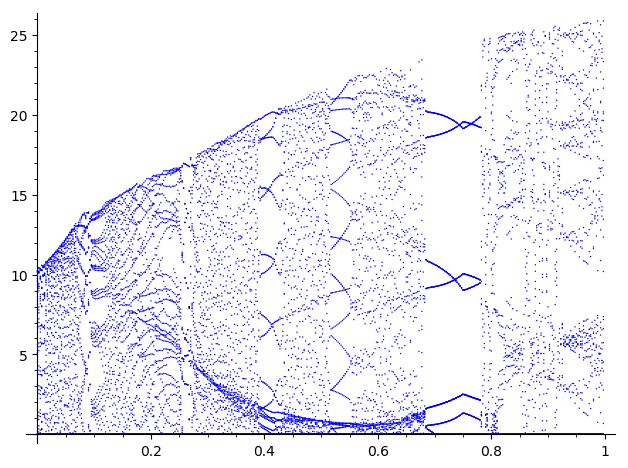
\includegraphics[scale=1.0]{example3_1.png}
\section*{Example 2, Using the plot2DGrayScale function}
I don't know why I called this function "grayscale" because it actually plots in color. 

This function is similar to the plotParamsLinear function as it plots a value of the system after a certain number of iterations vs. the paramaters used.
With this function the X and Y axis are two different parameter values that are chosen (here we have 'alpha' and 'beta') and a range for them to be plotted over.
The color of the plot at each point represents the value of a certain variable (in this case "FI") after a certain amount of iterations with the hotter colors 
being larger values and the cooler colors being smaller (sage automatically scales it so the lowest value is blue and the highest is red).
This function is kind of hard to experiment with as it will take a while to process if you want a quality image but you can get some pretty interesting pictures.
I noticed a lot of them look like clouds which maybe is related to the fact that weather also has chaotic behavior.
\linebreak
Code:
\begin{lstlisting}
plot2DGrayscale(Params(alpha = 0.40,
           			    beta = 0.0,
						theta = 0.2,
						Q = 0.3,
						RIO = 5 #for now, demand is constant
						),'alpha', 'beta', 0.4,0.8, "FI", 210, 100)
\end{lstlisting}
Output:
\linebreak
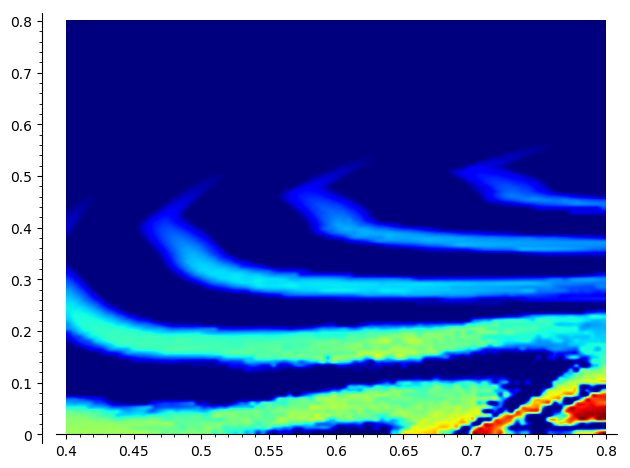
\includegraphics[scale=1.0]{example4_1.png}

\end{document}
